% convergence-rms/ag30_spline_warped.tex — generated by convergence/tools/rms_figure.py; do not edit.
% One panel (Sigma 14 mm lens, AprilGrid, Spline): the median per LM iteration of the detections' true reprojection error and of the held-out reprojection error on
% the high-precision target, both in px on one axis, its key under it. The axis box is \rcpanelwidth wide (\linewidth when the host
% does not define it) and is ALL of the picture's width (trim axis left / right): the y tick labels and the y label \rcpanelylabel
% stand out to its left, the last x tick label to its right — the host leaves room for them. The baseline is the picture's lower edge.
\providecommand{\rcpanelwidth}{\linewidth}\providecommand{\rcpanelylabel}{Median reprojection error [px]}%
\definecolor{rcdet}{HTML}{FF0000}\definecolor{rcchr}{HTML}{0000FF}%
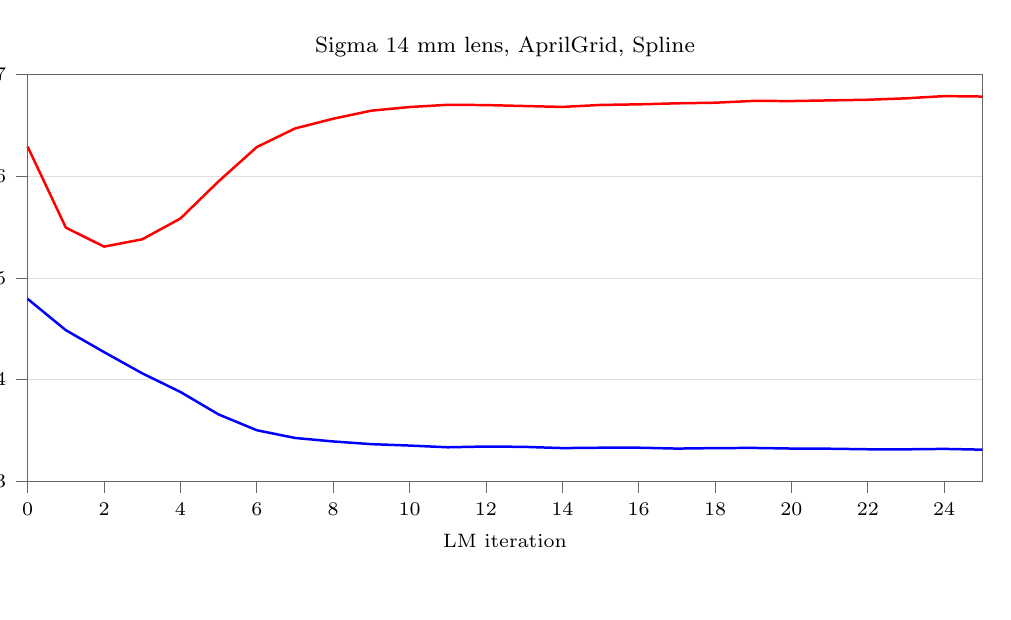
\begin{tikzpicture}[baseline=(current bounding box.south), trim axis left, trim axis right]
\begin{axis}[width=\rcpanelwidth, height=0.4259*\rcpanelwidth, scale only axis, xmin=0, xmax=25, ymin=0.3, ymax=0.7, ytick distance=0.1, tick label style={font=\scriptsize}, label style={font=\scriptsize}, tick align=outside, tick style={black!60, line width=0.3pt}, axis line style={black!60, line width=0.3pt}, scaled y ticks=false, title style={font=\footnotesize, yshift=-3pt}, title={Sigma 14 mm lens, AprilGrid, Spline}, xlabel={LM iteration}, xtick pos=left, ytick pos=left, ymajorgrids, grid style={black!12, line width=0.3pt}, clip=false, yticklabel style={/pgf/number format/fixed, /pgf/number format/precision=2}, ylabel={\rcpanelylabel}]
\addplot[rcchr, line width=0.9pt, no marks] coordinates {(0,0.479401) (1,0.448594) (2,0.427077) (3,0.406175) (4,0.387851) (5,0.365746) (6,0.350214) (7,0.342611) (8,0.33918) (9,0.336529) (10,0.335144) (11,0.333448) (12,0.334201) (13,0.333871) (14,0.332649) (15,0.333017) (16,0.333033) (17,0.332171) (18,0.332636) (19,0.33282) (20,0.332211) (21,0.332024) (22,0.331501) (23,0.331445) (24,0.331851) (25,0.331107)};
\addplot[rcdet, line width=0.9pt, no marks] coordinates {(0,0.629097) (1,0.549551) (2,0.530836) (3,0.538027) (4,0.558502) (5,0.595073) (6,0.628786) (7,0.647052) (8,0.656638) (9,0.664582) (10,0.668141) (11,0.670354) (12,0.670069) (13,0.669146) (14,0.668246) (15,0.670206) (16,0.670782) (17,0.671808) (18,0.67239) (19,0.674187) (20,0.674022) (21,0.674677) (22,0.675312) (23,0.676721) (24,0.678901) (25,0.678465)};
\end{axis}
% the key: centred under the axis box; it may be wider than the box, so it does not count for the picture's width (overlay) —
% the short invisible path keeps its height in the picture's bounding box
\path ([yshift=-0.5in-0.9ex]current axis.south) -- ++(0pt,2ex);
\end{tikzpicture}%
